\section{TODO Extending GP for more explainability}

In this section, the most important enhancements are presented, which have been added to the classical programming to make it even easier to explain.

\subsection{TODO Tree edit distance ted, apted}

The Tree Edit Distance (TED) was selected as basis measurement, as it fits all the requirements. The TED is a well-known problem from theoretical computer science which deals with how many changes there are between two trees to be compared:

``The tree-to-tree correction problem is to determine, for two labeled ordered trees {\tt{T}} and {\tt{T'}}, the distance from  T to T' as measured  by the minimum cost sequence of edit operations needed to transform  T into T'. The edit operations investigated allow changing one node of a tree into another node, deleting one node from a tree, or inserting a node  into a tree.'' \cite{tedOldestPaper}

The TED computes the minimum amount of delete, insert and rename steps that are needed to transform one tree (the origin tree) to the gp-candidate tree as can be seen in \ref{fig:TED_explain_operators}. Computing this distance is a challenge itself and was widely researched on. Thanks to numerous improvements made in the last years, the state of the art TED computation is robust and fast enough for evaluating numerous of gp-generated trees. \cite{tedAPTED1, tedAPTED2}

\begin{figure}
    \centering
    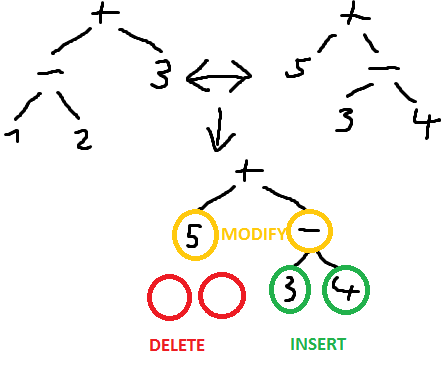
\includegraphics{img/general/ted_explain.png}
    \caption{Basic TED operators}
    \label{fig:TED_explain_operators}
\end{figure}


\subsubsection{TODO Fix nodes, Modifiable Nodes}

As a further possibility for recognizing the origin is, if the expert is very sure of his reasoning, to specify nodes that are logic wise sure as non-modifiable. These fix nodes are will remain unchanged throughout the whole evolutionary process. 


An example for a tree used in the mountain car problem can be seen in \ref{img:tree_modifiable_nodes}.

This significantly limits the genetic programming on the logical parts it can improve. It is also not a commonly used concept in genetic programming and the impacts on the genetic programming will be discussed and tested further this thesis. However, it definitely marks an explainable root structure that the programmer can understand and where he can be certain about.

\begin{figure}[ht]
	\centering
  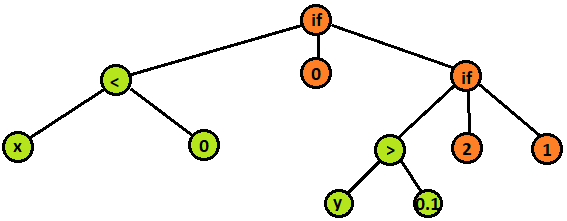
\includegraphics[scale=0.6]{img/trees/tree_modifiable_nodes.png}
	\caption{Red nodes have to stay the same, green ones can be modified}
	\label{img:tree_modifiable_nodes}
  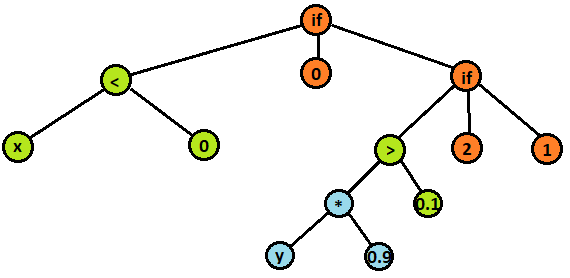
\includegraphics[scale=0.6]{img/trees/tree_modifiable_nodes_improved.png}
	\caption{The same tree with inserted nodes in blue}
	\label{img:tree_modifiable_nodes_modified}
\end{figure}

\subsubsection{TODO Explainable Genetic Programming}

The advantage of this is not only that the information (in the form of a program) is easier to understand. The complexity of the model is also only as great as the function it represents. After all, it is the function.
Nevertheless, one should not jump to hasty conclusions. The problems we are dealing with here are such that there is usually no simple solution. A program written by a computer, consisting of several hundred lines and largely consisting of parts that are not comprehensible to the developer, is as meaningful as a neural network. Developers sometimes have problems to reproduce their own code that they have written only one day before.

\subsection{TODO Explainable Neural Networks}


\begin{figure}[ht]
	\centering
  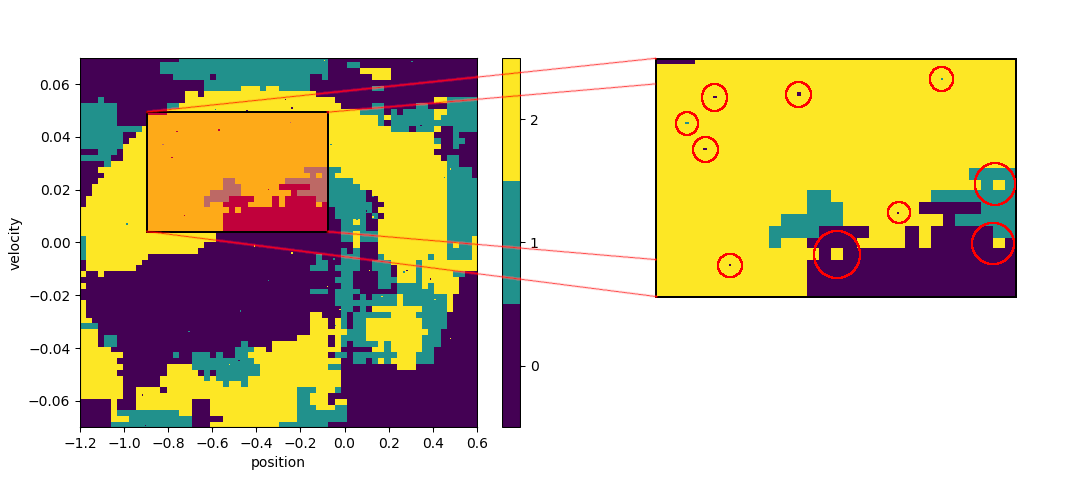
\includegraphics[width=1\textwidth]{img/MTC/sarsa_100_decision_plot.png}
	\caption{State-Action mapping on SARSA-policy with several arbitrary fragments}
	\label{img:SARSA-plot-fragments}
\end{figure}

\section{todo explainable visualisation}

The generated code can be presented to the expert as written code, mathematical expression or tree visualization. This is only a matter of taste and does not influence the real explainability of a program.

In general, tree visualizations offer the greatest possibilities. Not only do they offer a simple and clear representation, but special program parts can also be marked separately according to preference.

The special visualizations should help the developer to recognize patterns even better.

- What is left of the developer's core program is marked with a different color.

- Inputs have their own color

- Bool and Float are not distinguished